\documentclass{article}
\usepackage[utf8]{inputenc}
\usepackage[italian]{babel}
\usepackage{amsmath}
\usepackage{amssymb}
\usepackage{siunitx}
\usepackage{tabularray}
\usepackage{graphicx}
\usepackage{float}
\usepackage[bottom]{footmisc}
\usepackage[page]{appendix}
\usepackage[mathscr]{euscript}  % per il corsivo
\usepackage[labelformat=simple, justification=centering]{subfig}
\renewcommand{\thesubfigure}{}
\newcommand*{\diam}{\varnothing}
\newcommand*{\best}[1]{{#1}_\text{best}}
\newcommand*{\bestp}[1]{{\left(#1\right)}_\text{best}}
\newcommand*{\pbest}[1]{\left({#1}_\text{best}\right)}
\newcommand*{\pbestp}[1]{\left({\left(#1\right)}_\text{best}\right)}
\newcommand*{\errrel}[1]{\frac{\delta #1}{{#1}_\text{best}}}
\title{
  Laboratorio di Fisica 1\\
  R11: Calorimetro ad azoto liquido
}
\author{Gruppo 15: Bergamaschi Riccardo, Graiani Elia, Moglia Simone}
\date{14/05/2024 – 21/05/2024}
\makeindex
\begin{document}

\maketitle

\begin{abstract}
  Mediante un calorimetro ad azoto liquido, il gruppo di lavoro
  ha misurato i calori specifici di quattro campioni;
  preliminarmente, è stato necessario determinare il
  calore latente di vaporizzazione dell'azoto.
\end{abstract}

\setcounter{section}{-1}
\section{Materiali e strumenti di misura utilizzati}
\begin{center}
\begin{tblr}{
  width=\textwidth,
  colspec={ X[2,m,j]X[1,m,c]X[1,m,c]X[1,m,c] },
  vlines,
}
  \hline
  \textbf{Strumento di misura} & \textbf{Soglia} & \textbf{Portata} & \textbf{Sensibilità} \\
  \hline
  Amperometro & $\qty{0.001}{A}$ & N./A. & $\qty{0.001}{A}$ \\
  \hline[dashed]
  Voltmetro & $\qty{0.01}{V}$ & N./A. & $\qty{0.01}{V}$ \\
  \hline[dashed]
  Cronometro & $\qty{0.01}{s}$ & $\qty{99.99}{s}$ & $\qty{0.01}{s}$ \\
  \hline[dashed]
  Bilancia di precisione & $\qty{0.01}{g}$ & $\qty{4000.0}{g}$ &
    $\qty{0.01}{g}$\footnotemark[1] \\
  \hline
\end{tblr}
\footnotetext[1]{
  Per misure superiori a $\qty{2000.00}{g}$, la sensibilità
  è $\qty{0.1}{g}$
}
\begin{tblr}{
  width=\textwidth,
  colspec={ X[m,j]X[3,m,j] },
  vlines,
}
  \hline
  \textbf{Altro} & \textbf{Descrizione/Note} \\
  \hline
  Calorimetro & {
    Quasi adiabatico,
    dotato di un coperchio con un foro centrale per potervi immergere
    i materiali e permettere la fuoriuscita dell'azoto gassoso.
  } \\
  \hline[dashed]
  Azoto liquido & Contenuto nel calorimetro \\
  \hline[dashed]
  Resistenza & {
    Fissata all'interno del coperchio, fornisce calore all'azoto liquido.
  } \\
  \hline[dashed]
  Videocamera & {
    Utilizzata per acquisire i dati mostrati dal
    cronometro e della bilancia di precisione
    contemporaneamente.
  } \\
  \hline[dashed]
  Generatore & {
    Fornisce corrente elettrica al circuito, composto dall'amperometro
    (collegato in serie) e da voltmetro e resistenza (collegati in
    parallelo).
  } \\
  \hline[dashed]
  Quattro campioni metallici noti & { Li chiameremo $\Xi,\Delta,\aleph,\nabla$. } \\
  \hline
\end{tblr}
\end{center}

\pagebreak

\section{Misura del calore latente di vaporizzazione dell'azoto}

\subsection{Esperienza e procedimento di misura}

\begin{enumerate}
  \item
    Posto il calorimetro sopra alla bilancia di precisione, avviamo
    l'acquisizione del filmato.
  \item
    Dopo almeno una decina di secondi, accendiamo il generatore
    in modo da fornire calore all'azoto per mezzo della resistenza.
  \item
    Mediante il voltmetro e l'amperometro, misuriamo, rispettivamente,
    la differenza di potenziale ($\Delta V$) ai capi della resistenza
    e l'intensità di corrente ($i$) sviluppate dal generatore\footnote{
In entrambe le misurazioni, abbiamo rilevato
$\Delta V = (3.27\pm0.01)\,\unit{V}$ e $i = (1.636\pm0.001)\,\unit{A}$.
    }.
  \item
    Passato circa un minuto, spegniamo il generatore per interrompere
    lo scambio di calore e, dopo almeno un'altra decina di secondi,
    terminiamo la registrazione del filmato.
\end{enumerate}

Il gruppo di lavoro ha effettuato questi passaggi due volte:
la prima, chiudendo il foro del coperchio con un tappo;
la seconda, lasciandolo aperto.

\subsection{Analisi dei dati raccolti}

Essendo l'azoto a temperatura di ebollizione, possiamo esprimere la
quantità di calore assorbito ($\delta Q$) in un intervallo di tempo
$\Delta t$ in funzione della massa di azoto evaporata ($-\Delta m$):
\[\delta Q = - \lambda_\text{vap} \Delta m\] dove la costante
$\lambda_\text{vap}$ è detta “calore latente di vaporizzazione”.

Assumendo le dispersioni di energia trascurabili, possiamo
considerare $\delta Q$ pari al calore sviluppato dalla resistenza per
effetto Joule. Vale allora:
\[ \delta Q = \mathscr{P}\cdot\Delta t = i\cdot\Delta V\cdot\Delta t\]

da cui:
\[
  \lambda_\text{vap} = \frac{i\cdot\Delta V\cdot\Delta t}{-\Delta m}
    = \frac{i\cdot\Delta V}{-\,\gamma}
  \qquad \text{avendo posto} \quad
  \gamma = \frac{\Delta m}{\Delta t}.
\]

Visionando il filmato, il gruppo di lavoro ha raccolto, a intervalli
di tempo regolari, la misura della massa di azoto liquido indicata
dalla bilancia.

Chiaramente, non essendo il calorimetro perfettamente adiabatico,
la massa di azoto diminuisce anche quando la resistenza è spenta.
Per tenere conto di questo errore sistematico, abbiamo effettuato
tre regressioni lineari (con coefficienti angolari $\alpha_1,\beta,\alpha_2$)
sui dati raccolti, rispettivamente prima,
durante e dopo lo scambio di calore con la resistenza. Abbiamo quindi calcolato:
\[\gamma = \beta - \frac{\alpha_1 + \alpha_2}{2}.\]

\pagebreak
Di seguito riportiamo graficamente i dati acquisiti, accompagnati dalle rette
di regressione e dai valori di $\gamma$ e $\lambda_\text{vap}$ calcolati.

\vspace{2mm}
\emph{
  \textbf{Nota.} La struttura di entrambi i grafici è la seguente:
  \begin{itemize}
    \item in blu, i dati raccolti con la resistenza accesa e la
      relativa retta di regressione (la cui zona di incertezza,
      estremamente ridotta, è rappresentata in azzurro);
    \item in rosso, i dati raccolti con la resistenza spenta e le
      rispettive rette di regressione (le cui zone di incertezza
      sono rappresentate in rosa);
    \item sono inoltre riportate le barre di errore,
      tuttavia così ridotte da risultare invisibili.
  \end{itemize}
}

\subsubsection{Prima acquisizione: foro chiuso}
\begin{figure}[H]
  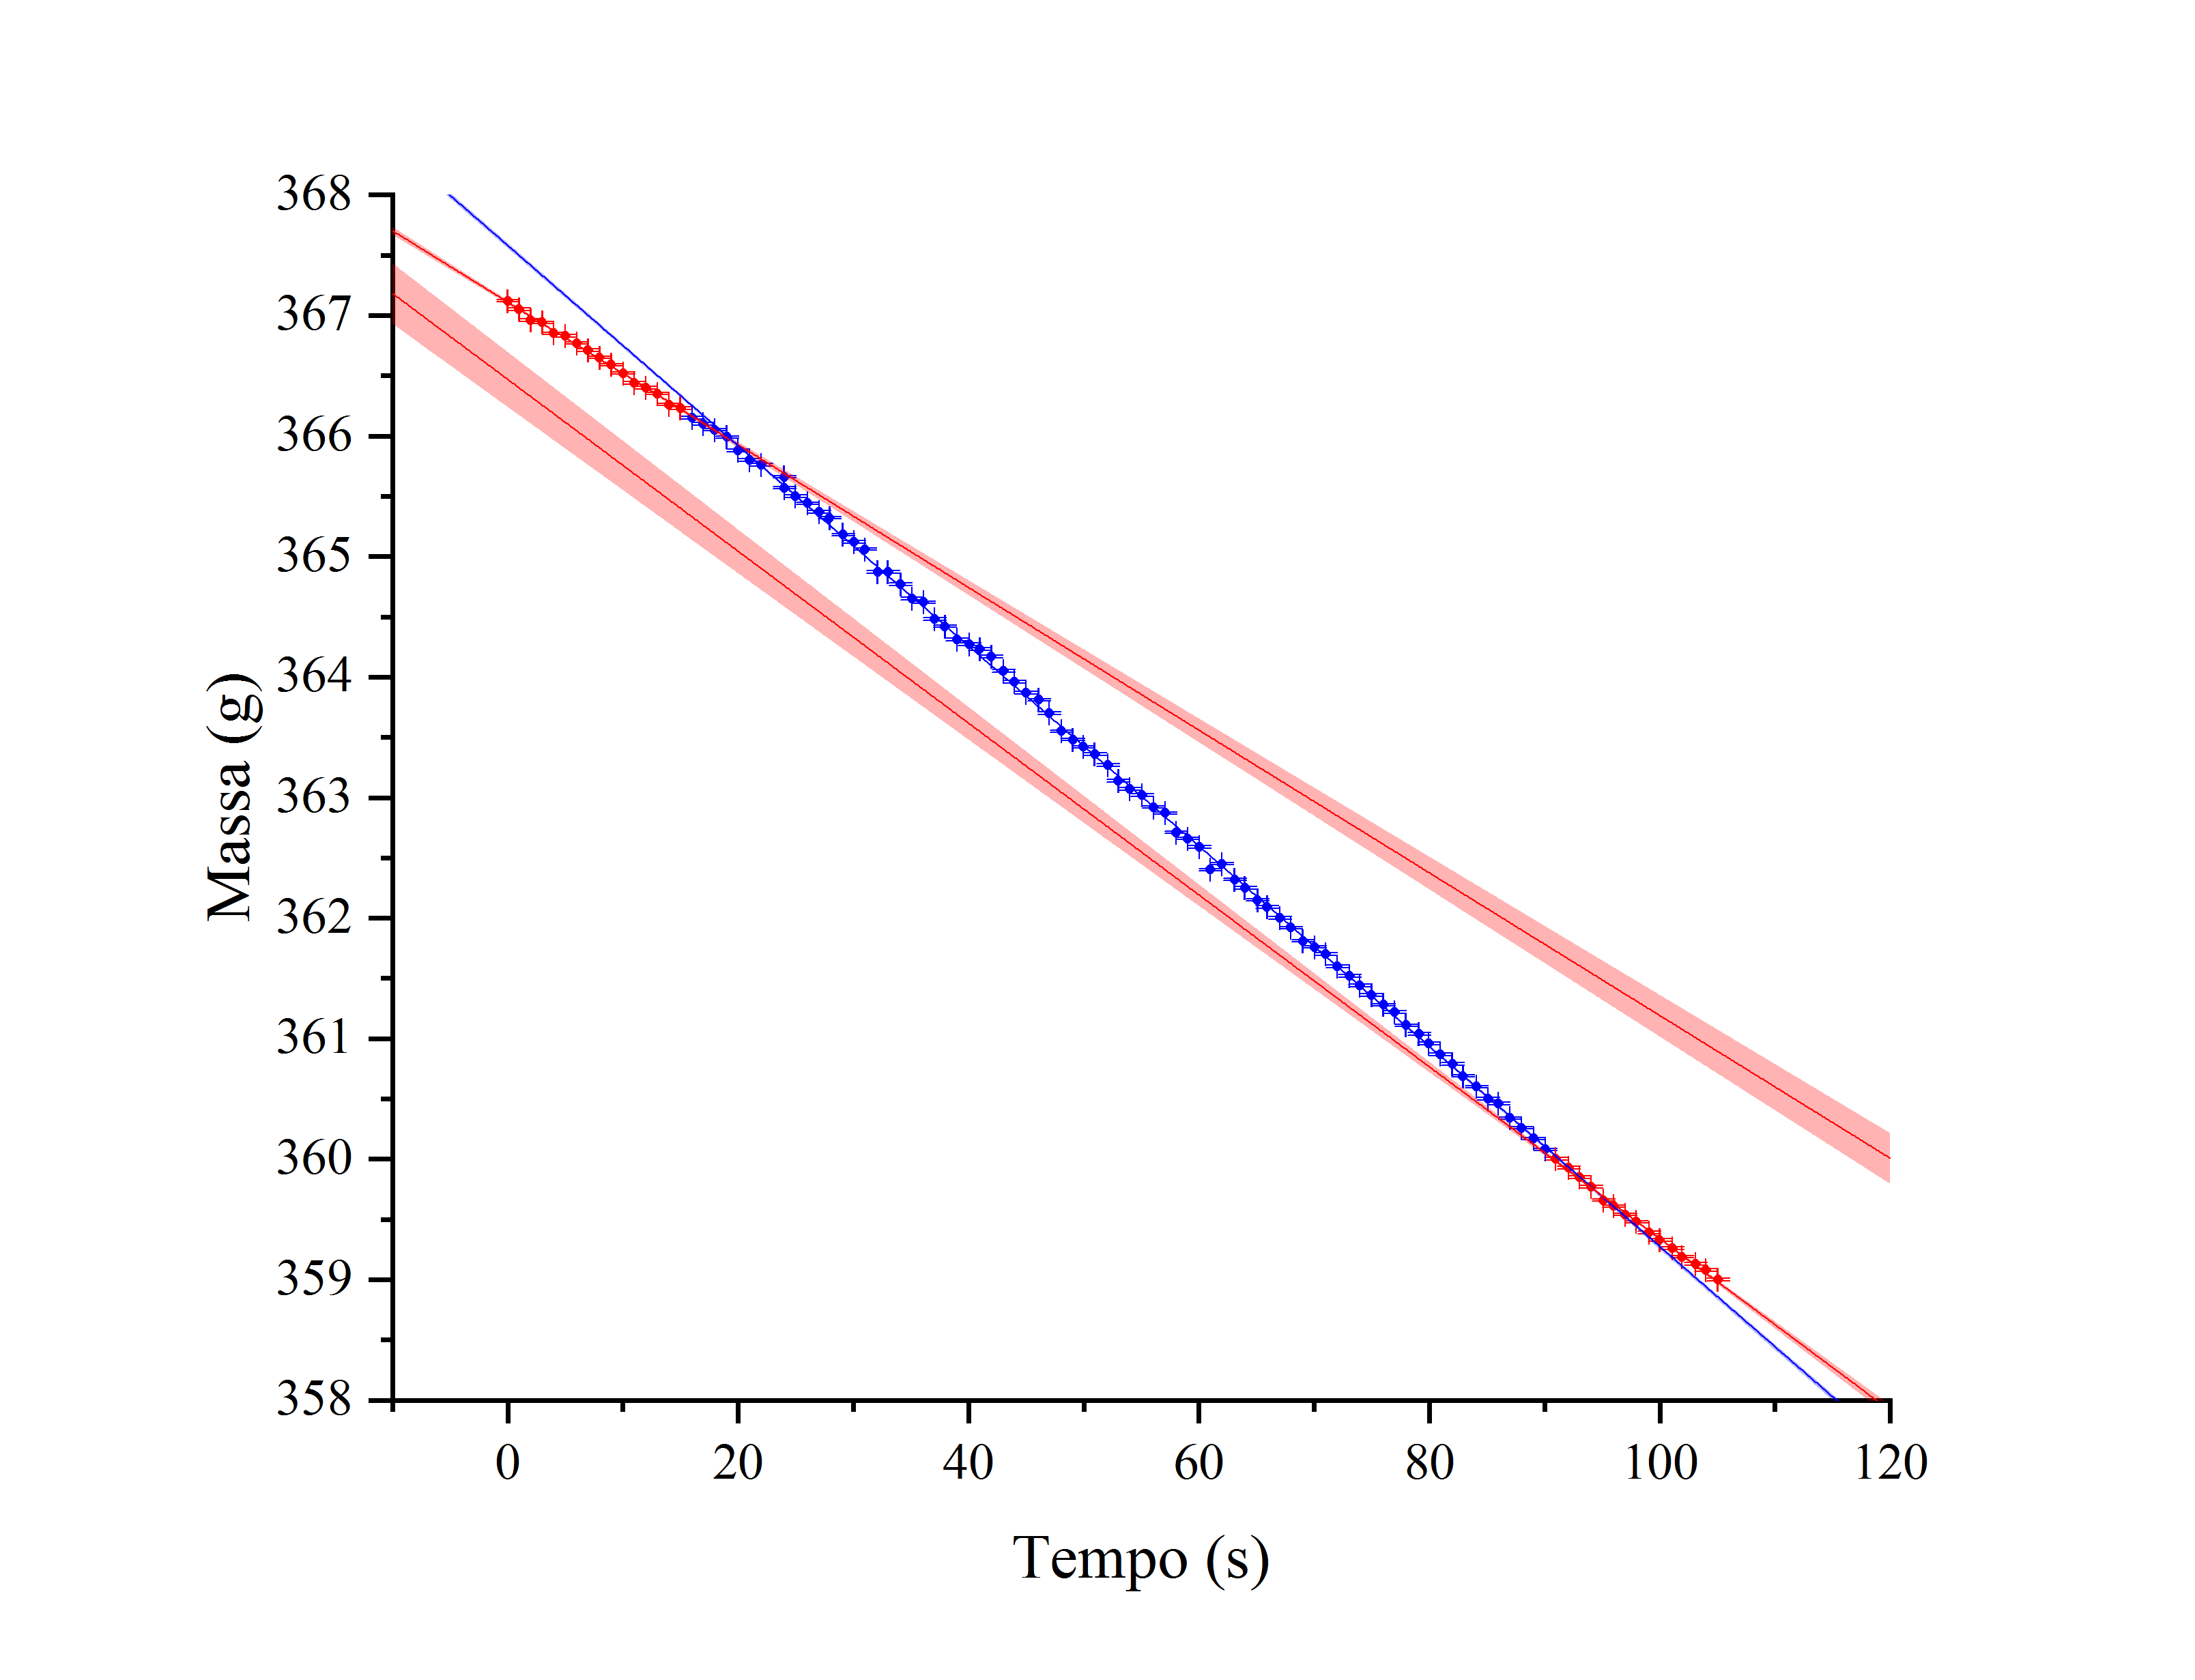
\includegraphics[trim={2.5cm 0.6cm 3cm 1cm},clip,width=\textwidth]{img/g_azoto2.png}
\end{figure}
\[\begin{aligned}
  \alpha_{1,\text{chiuso}} &= (-59.2\pm0.5)\cdot10^{-6}\,\unit{kg\per s}
  \qquad
  \beta_{\text{chiuso}}\!\!\!\!&=(-&83.06\pm0.05)\cdot10^{-6}\,\unit{kg\per s}
  \\
  \alpha_{2,\text{chiuso}} &= (-71.3\pm0.5)\cdot10^{-6}\,\unit{kg\per s}
  \qquad
  \gamma_\text{chiuso}\!\!\!\!&=(-&17.8\pm0.6)\cdot10^{-6}\,\unit{kg\per s}
\end{aligned}\]
\[
  \lambda_\text{vap,chiuso} = (3.00\pm0.11)\cdot10^5\,\unit{J \per kg}
\]

\pagebreak
\subsubsection{Seconda acquisizione: foro aperto}
\begin{figure}[H]
  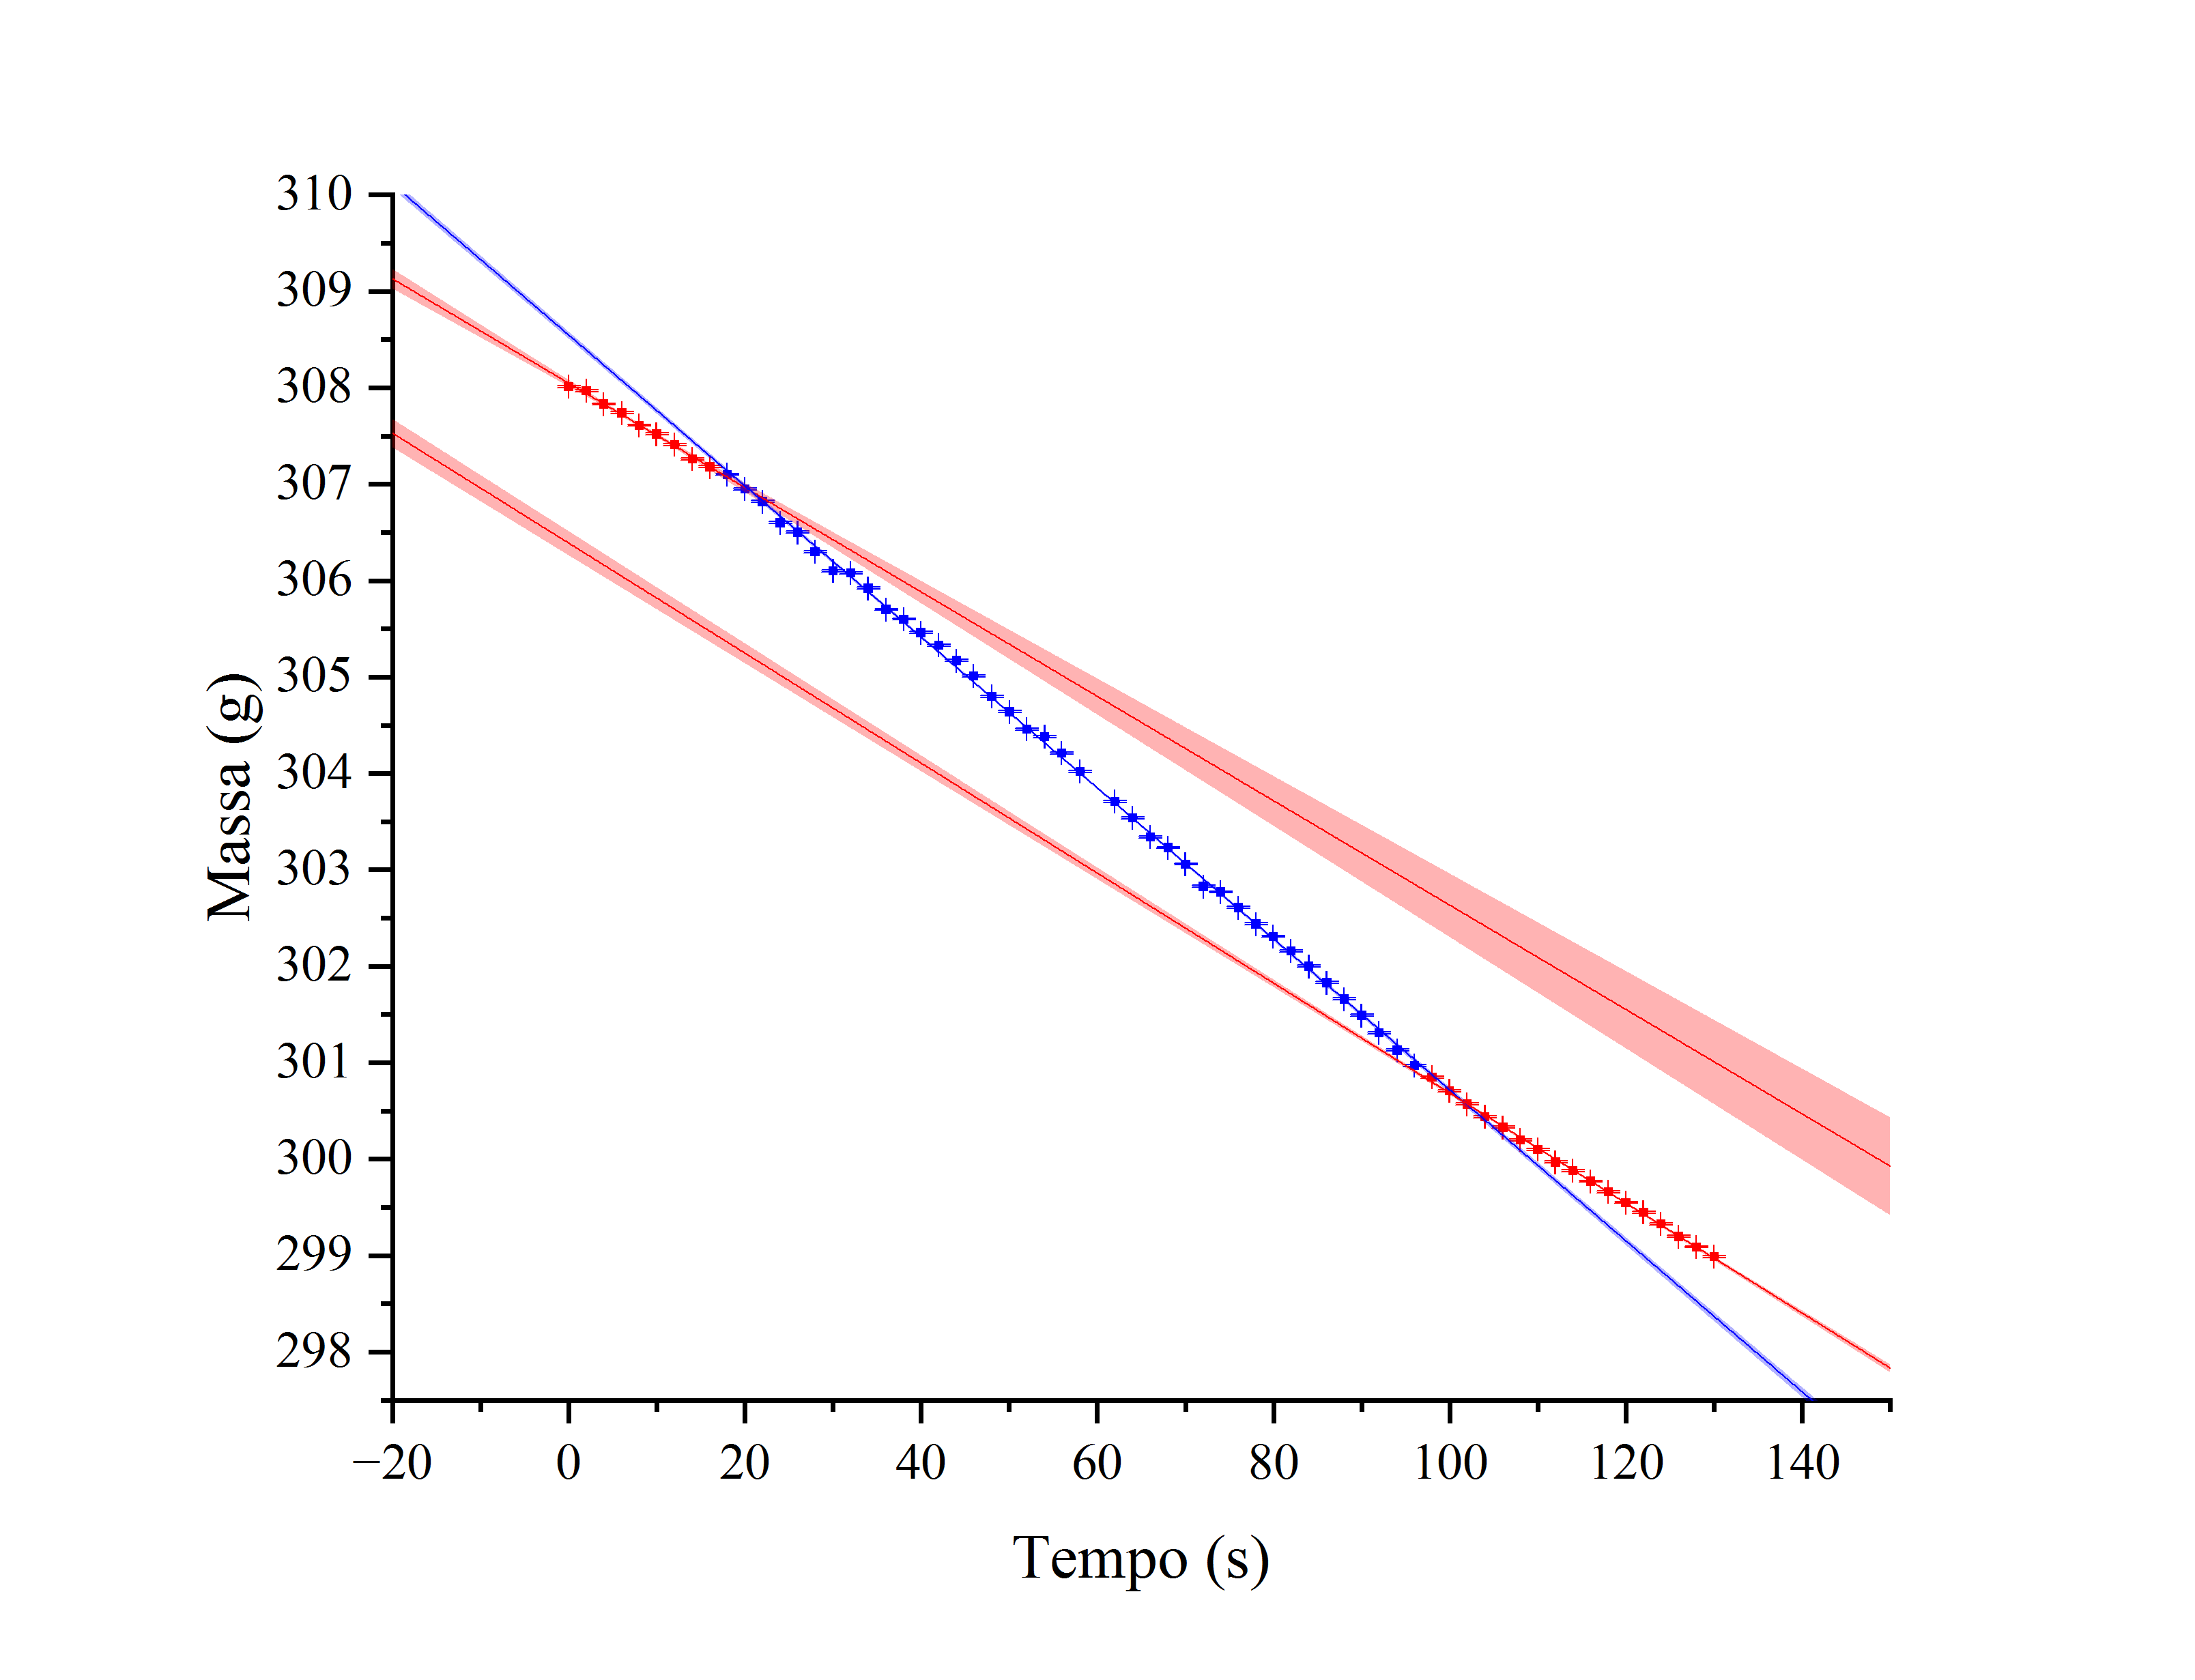
\includegraphics[trim={2.5cm 0.6cm 3cm 1cm},clip,width=\textwidth]{img/g_azoto3.png}
\end{figure}
\[\begin{aligned}
  \alpha_{1,\text{aperto}} &= (-54.1\pm0.6)\cdot10^{-6}\,\unit{kg\per s}
  \qquad
  \beta_{\text{aperto}}\!\!\!\!&=(-&78.28\pm0.07)\cdot10^{-6}\,\unit{kg\per s}
  \\
  \alpha_{2,\text{aperto}} &= (-57.0\pm0.2)\cdot10^{-6}\,\unit{kg\per s}
  \qquad
  \gamma_\text{aperto}\!\!\!\!&=(-&22.7\pm0.5)\cdot10^{-6}\,\unit{kg\per s}
\end{aligned}\]
\[
  \lambda_\text{vap,aperto} = (2.35\pm0.06)\cdot10^5\,\unit{J \per kg}
\]

\subsection{Conclusioni}
Confrontando i due valori di $\lambda_\text{vap}$ così ottenuti
con il valore atteso $\lambda_\text{vap,atteso} =
(1.9856\pm0.0001)\cdot10^5\,\unit{J\per kg}$,
possiamo osservare che nessuno dei due risulta compatibile con
quest'ultimo.

\vspace{2mm}
Per quanto riguarda $\lambda_\text{vap,chiuso}$, il gruppo di
lavoro ritiene che la presenza del tappo abbia impedito a una
parte significativa dell'azoto gassoso di fuoriuscire dal sistema,
portando la bilancia a misurare, in ogni momento, una massa di
azoto superiore a quella ancora in fase liquida. Ma, soprattutto,
la variazione di massa rispetto al tempo misurata mediante la
retta di regressione è risultata essere minore di quella effettiva,
portandoci a sovrastimare $\lambda_\text{vap}$ (ricordiamo che
$\gamma$ è al denominatore).

Questa ipotesi è coerente col fatto che $\lambda_\text{vap,aperto}$,
pur risultando anch'esso non compatibile, si avvicina di più al valore
di $\lambda_\text{vap,atteso}$.

\vspace{2mm}
Invece, riguardo a $\lambda_\text{vap,aperto}$, il gruppo di
lavoro ritiene che, durante l'esperienza, la resistenza non fosse
completamente immersa nell'azoto liquido: di conseguenza, parte
del calore sviluppato per effetto Joule è stato disperso,
probabilmente assorbito dall'azoto già in fase gassosa.
Di conseguenza, nell'analisi di cui sopra il calore assorbito
dall'azoto è stato sovrastimato e, con esso, anche
$\lambda_\text{vap}$.

Questa ipotesi è sostenuta dal fatto che, come è possibile
osservare dal grafico, la massa totale iniziale di azoto si
aggirava attorno ai $\qty{308}{g}$, quando il calorimetro ne
avrebbe potuto contenere ben di più.

\section{Misura dei calori specifici dei campioni}

\subsection{Esperienza e procedimento di misura}

Per ogni campione:
\begin{enumerate}
  \item
    Ne misuriamo la massa $\mu$ mediante la bilancia di precisione.
  \item
    Dopo aver posizionato il calorimetro sopra alla bilancia di precisione,
    avviamo l'acquisizione del filmato.
  \item
    Dopo circa una decina di secondi, inseriamo il campione nel calorimetro
    tramite il foro nel coperchio, fissandolo con il tappo.
  \item
    Attesi non meno di due minuti, per assicurarci che lo scambio di calore con
    l'azoto sia terminato da almeno una decina di secondi, interrompiamo
    la registrazione.
\end{enumerate}

\subsection{Analisi dei dati raccolti}
Analogamente a quanto detto prima, possiamo esprimere la quantità di calore
assorbito dall'azoto come:
\[
  \delta Q = - \lambda_\text{vap} \Delta m.
\]

Assumendo le dispersioni di energia trascurabili, possiamo
considerare $\delta Q$ pari al calore ceduto dal campione, che
passa da temperatura ambiente $T_\text{amb} = (25\pm1)\,\unit{\degree C}$
alla temperatura di equilibrio
$T_\text{eq} = T_\text{eb,azoto} = -\qty{195.80}{\degree C}$.
Vale allora\footnote{
  In realtà il calore specifico $c(T)$ di un materiale dipende dalla temperatura,
  mentre qua lo stiamo trattando come costante: in questa sede, con il simbolo $c$
  indicheremo infatti una stima della “media” di $c(T)$ sull'intervallo di
  temperature considerato $[T_\text{eb,azoto}, T_\text{amb}]$.
}:
\[\qquad
  \delta Q = c\,\mu\,\Delta T \qquad\text{con}\quad
  \Delta T = T_\text{amb} - T_\text{eb,azoto} = (221\pm1)\,\unit{K},
\]
dove $\mu$ è la massa del campione.

Risolvendo in $c$ si ottiene:
\[
  c = -\frac{\lambda_\text{vap}\,\Delta m}{\mu\,\Delta T}
    = -\frac{\lambda_\text{vap}\,\gamma\,\Delta t}{\mu\,\Delta T}
  \qquad \text{avendo posto} \quad
  \gamma = \frac{\Delta m}{\Delta t}.
\]

Visionando il filmato, il gruppo di lavoro ha raccolto, a intervalli
di tempo regolari, la misura della massa del sistema indicata
dalla bilancia.

Il valore di $\gamma$ è stato quindi calcolato come nella prima parte
dell'esperienza:
\[\gamma = \beta - \frac{\alpha_1 + \alpha_2}{2}.\]

% TODO: Considerare una nota a piè di pagina
$\Delta t$, l'intervallo di tempo dello scambio di calore,
è stato invece calcolato come differenza fra i valori indicati
dal cronometro nell'istante di termine dello scambio di calore
(individuabile dal grafico) e nel momento di immersione del campione
nel calorimetro (stimabile, con un certo errore, sulla base del filmato).

Di seguito riportiamo graficamente i dati acquisiti, accompagnati dalle rette
di regressione e dai valori di $\gamma$ e $\Delta t$ ottenuti.

\vspace{2mm}
\emph{
  \textbf{Nota.} La struttura di entrambi i grafici è la seguente:
  \begin{itemize}
    \item in blu, i dati raccolti durante lo scambio di calore e la
      relativa retta di regressione (la cui zona di incertezza,
      estremamente ridotta, è rappresentata in azzurro);
    \item in rosso, i dati raccolti prima e dopo lo scambio di calore
      e le rispettive rette di regressione (le cui zone di incertezza
      sono rappresentate in rosa);
    \item sono inoltre riportate le barre di errore,
      tuttavia così ridotte da risultare invisibili.
  \end{itemize}
}


\begin{figure}[H]
  \subfloat[][
    Campione $\Xi$ (piombo) \\
    $\gamma=(-35\pm7)\cdot10^{-6}\,\unit{kg\per s}$ \\
    $\Delta t = (62\pm3)\,\unit{s}$
  ]{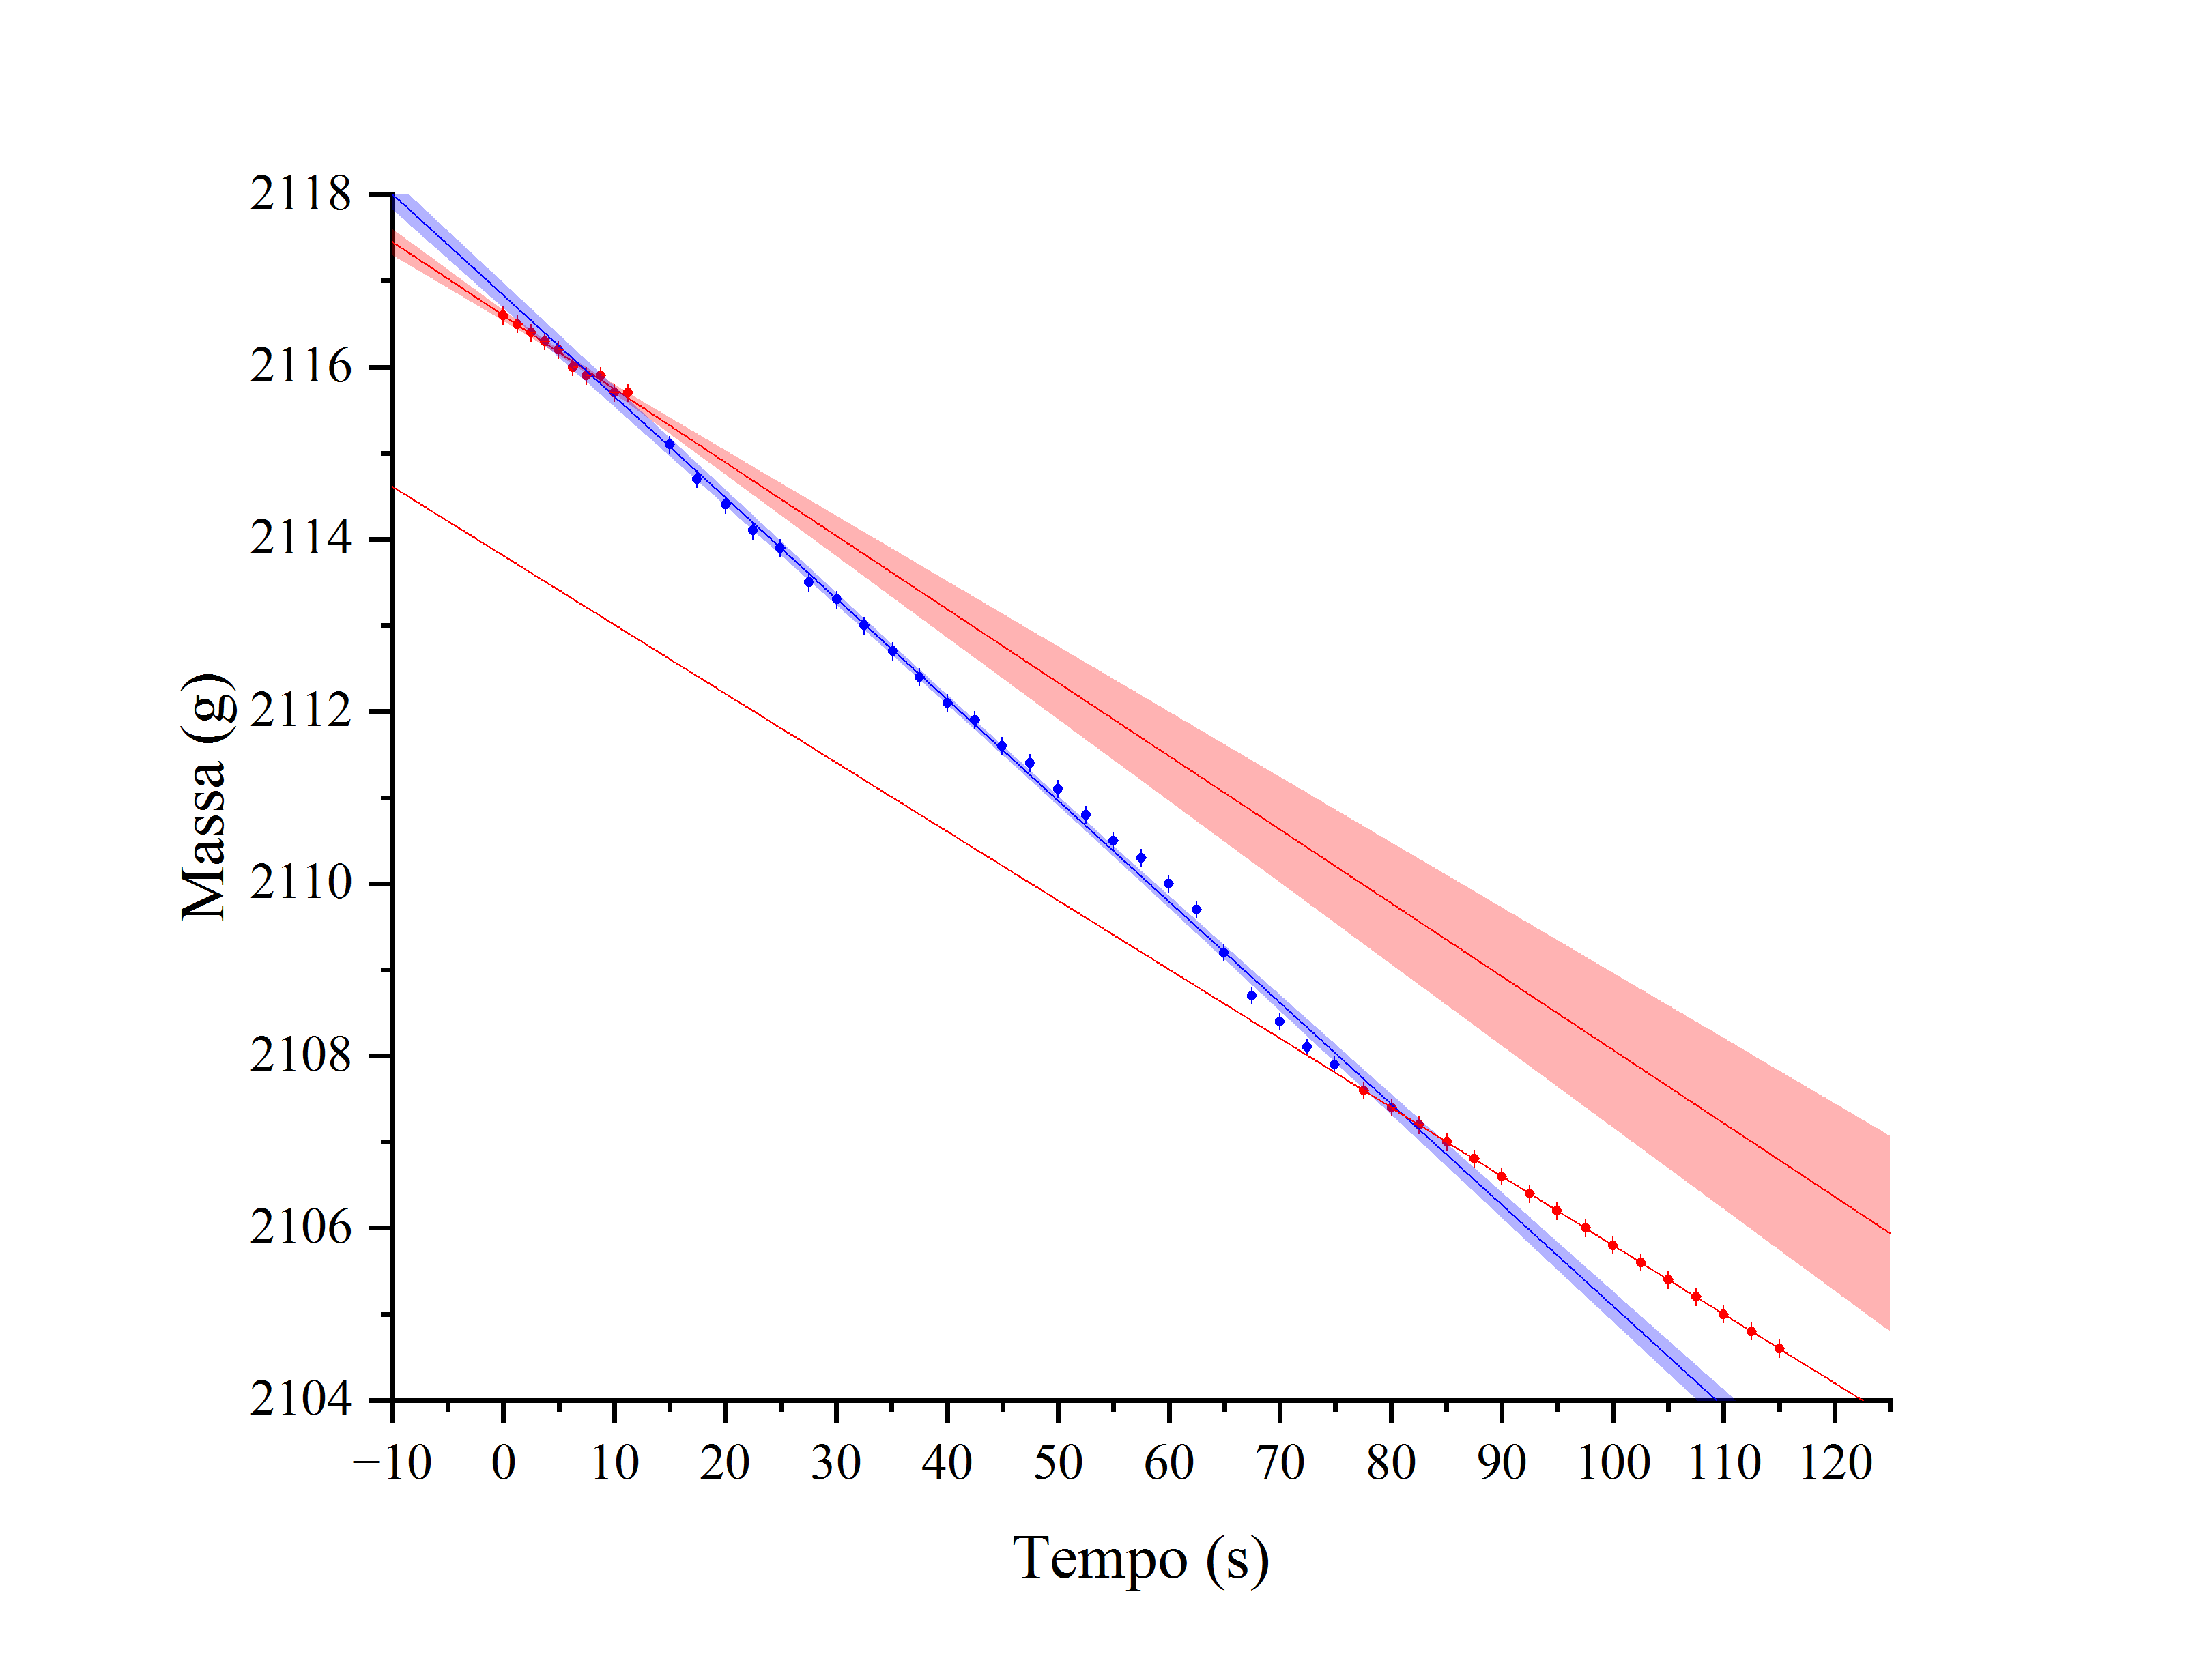
\includegraphics[trim={2cm 0.6cm 3.5cm 1cm},clip,width=.49\textwidth]{img/g_piombo.png}}\hfil
  \subfloat[][
    Campione $\Delta$ (ottone) \\
    $\gamma=(-92\pm3)\cdot10^{-6}\,\unit{kg\per s}$ \\
    $\Delta t = (90\pm5)\,\unit{s}$
  ]{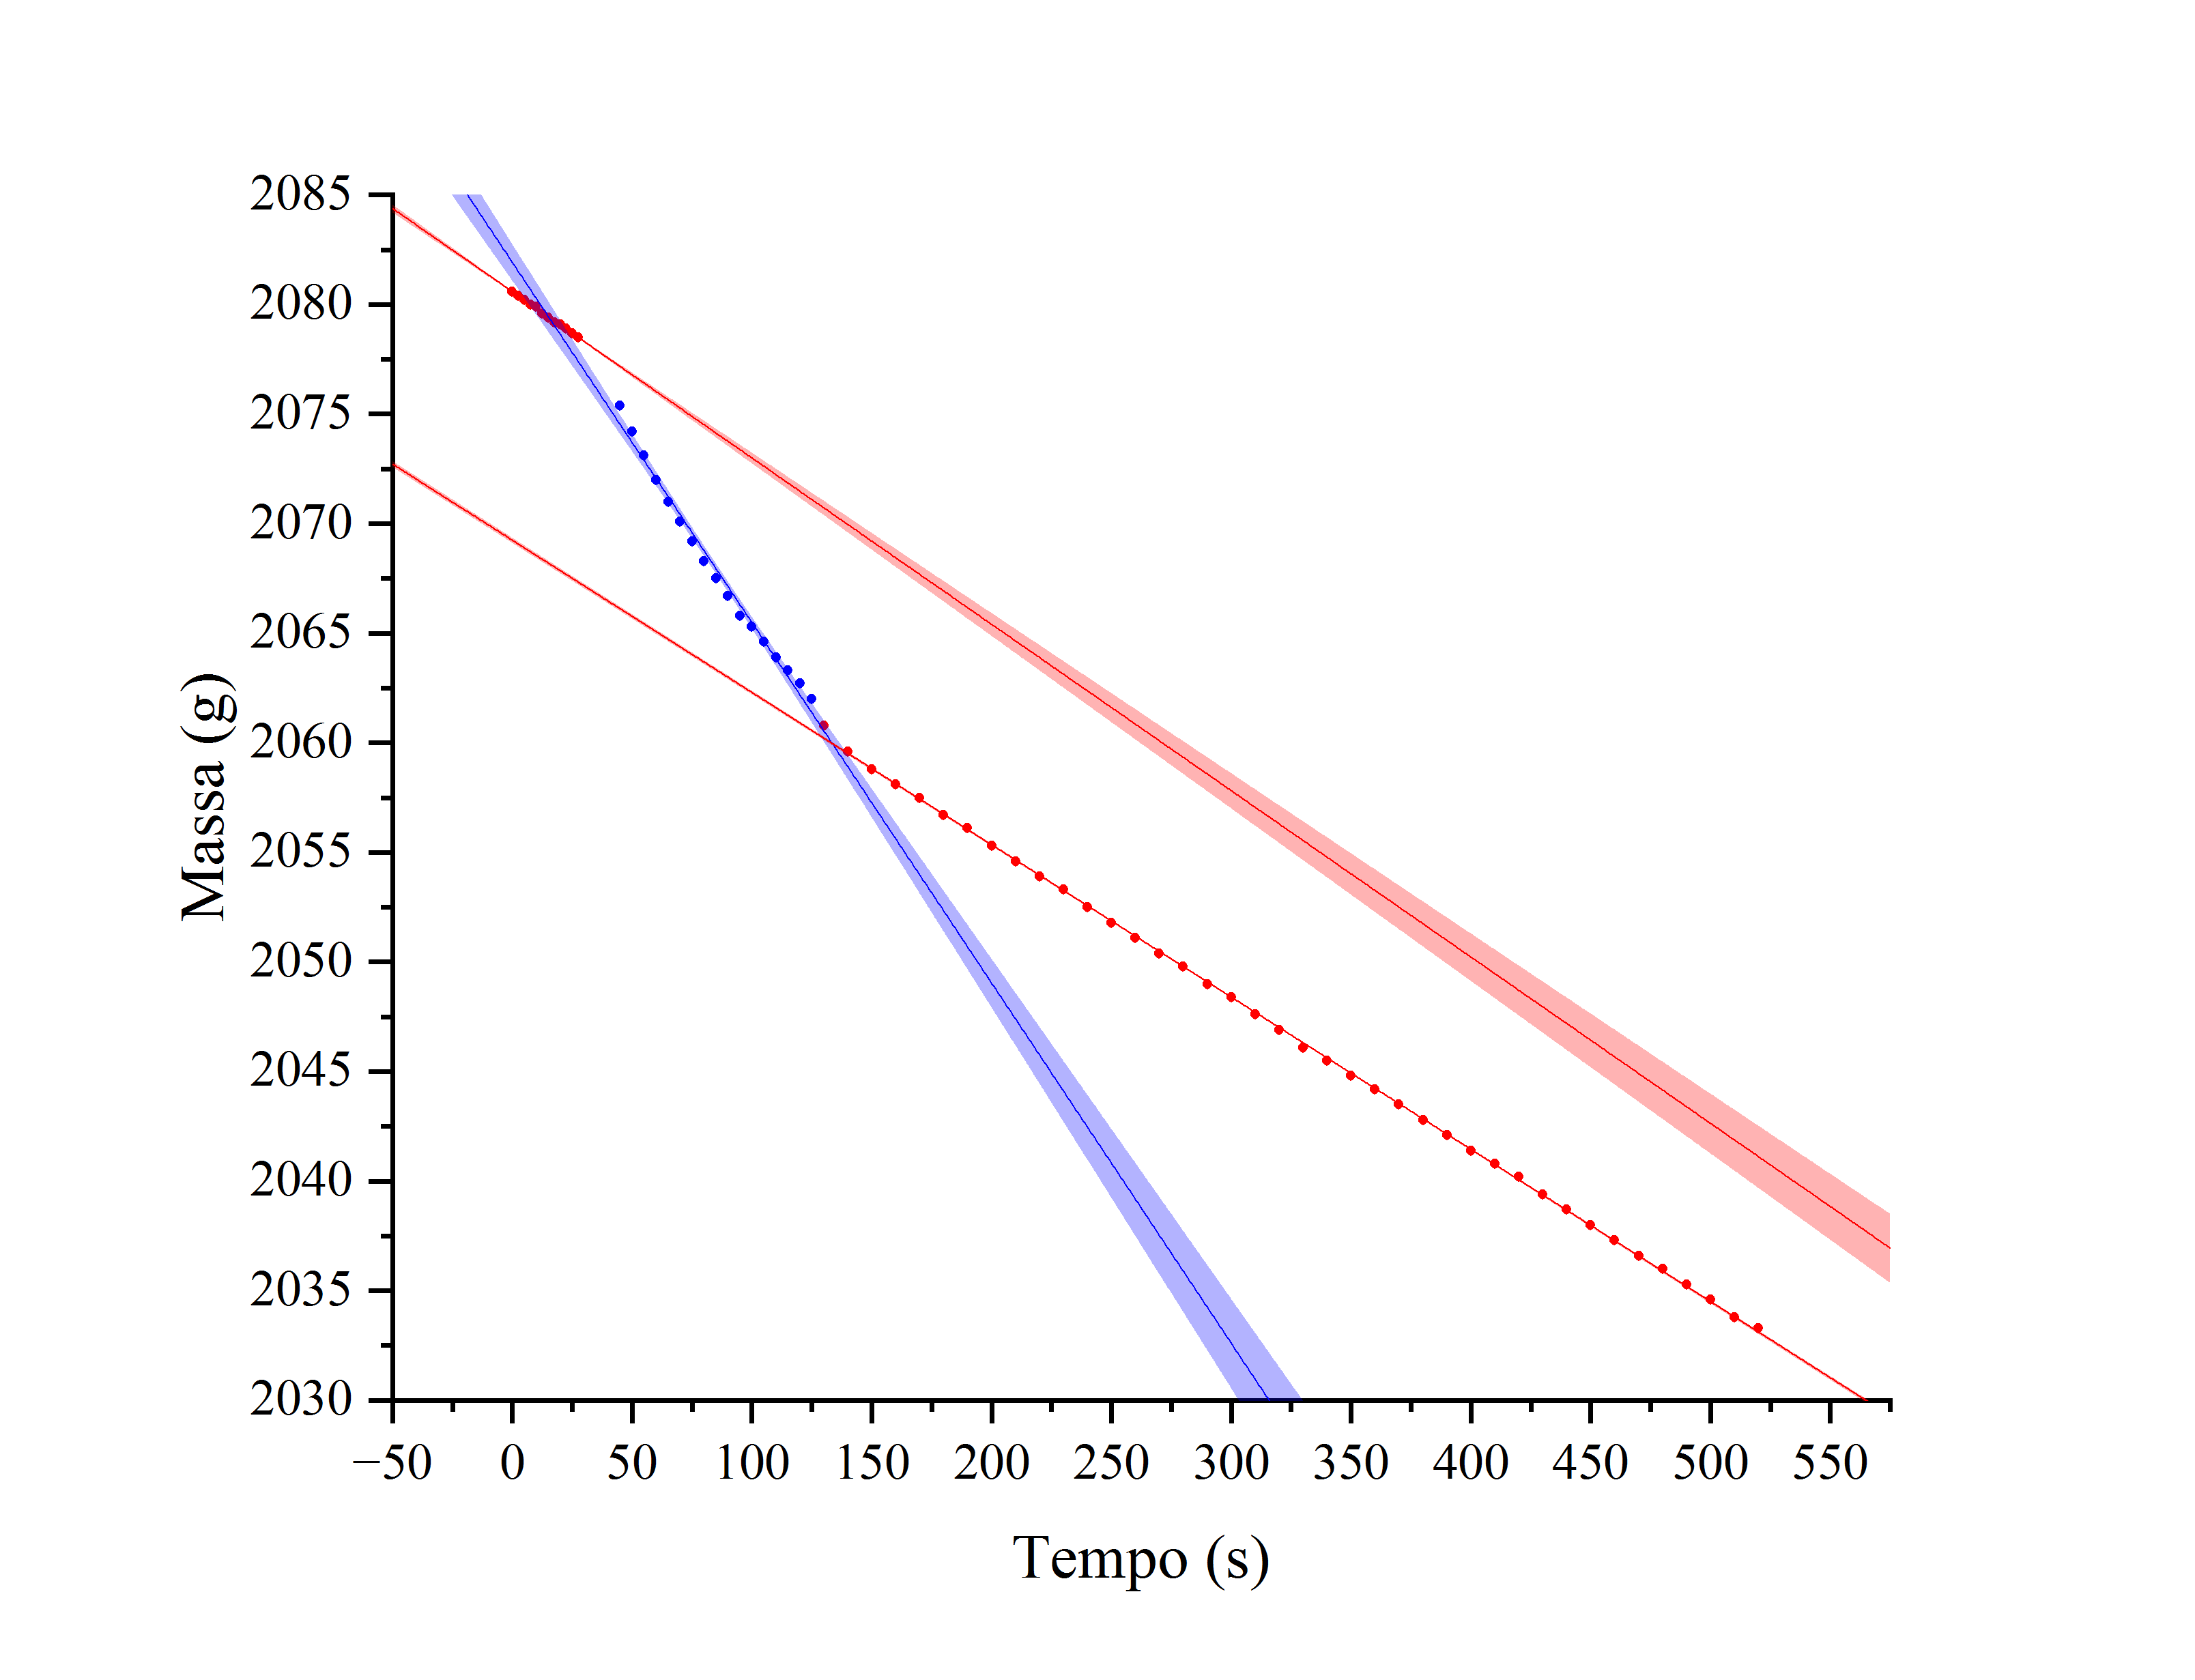
\includegraphics[trim={2cm 0.6cm 3.5cm 1cm},clip,width=.49\textwidth]{img/g_ottone.png}}\hfil
\end{figure}\begin{figure}[H]
  \subfloat[][
    Campione $\aleph$ (alluminio) \\
    $\gamma=(-91.4\pm0.4)\cdot10^{-6}\,\unit{kg\per s}$ \\
    $\Delta t = (73.5\pm1.3)\,\unit{s}$
  ]{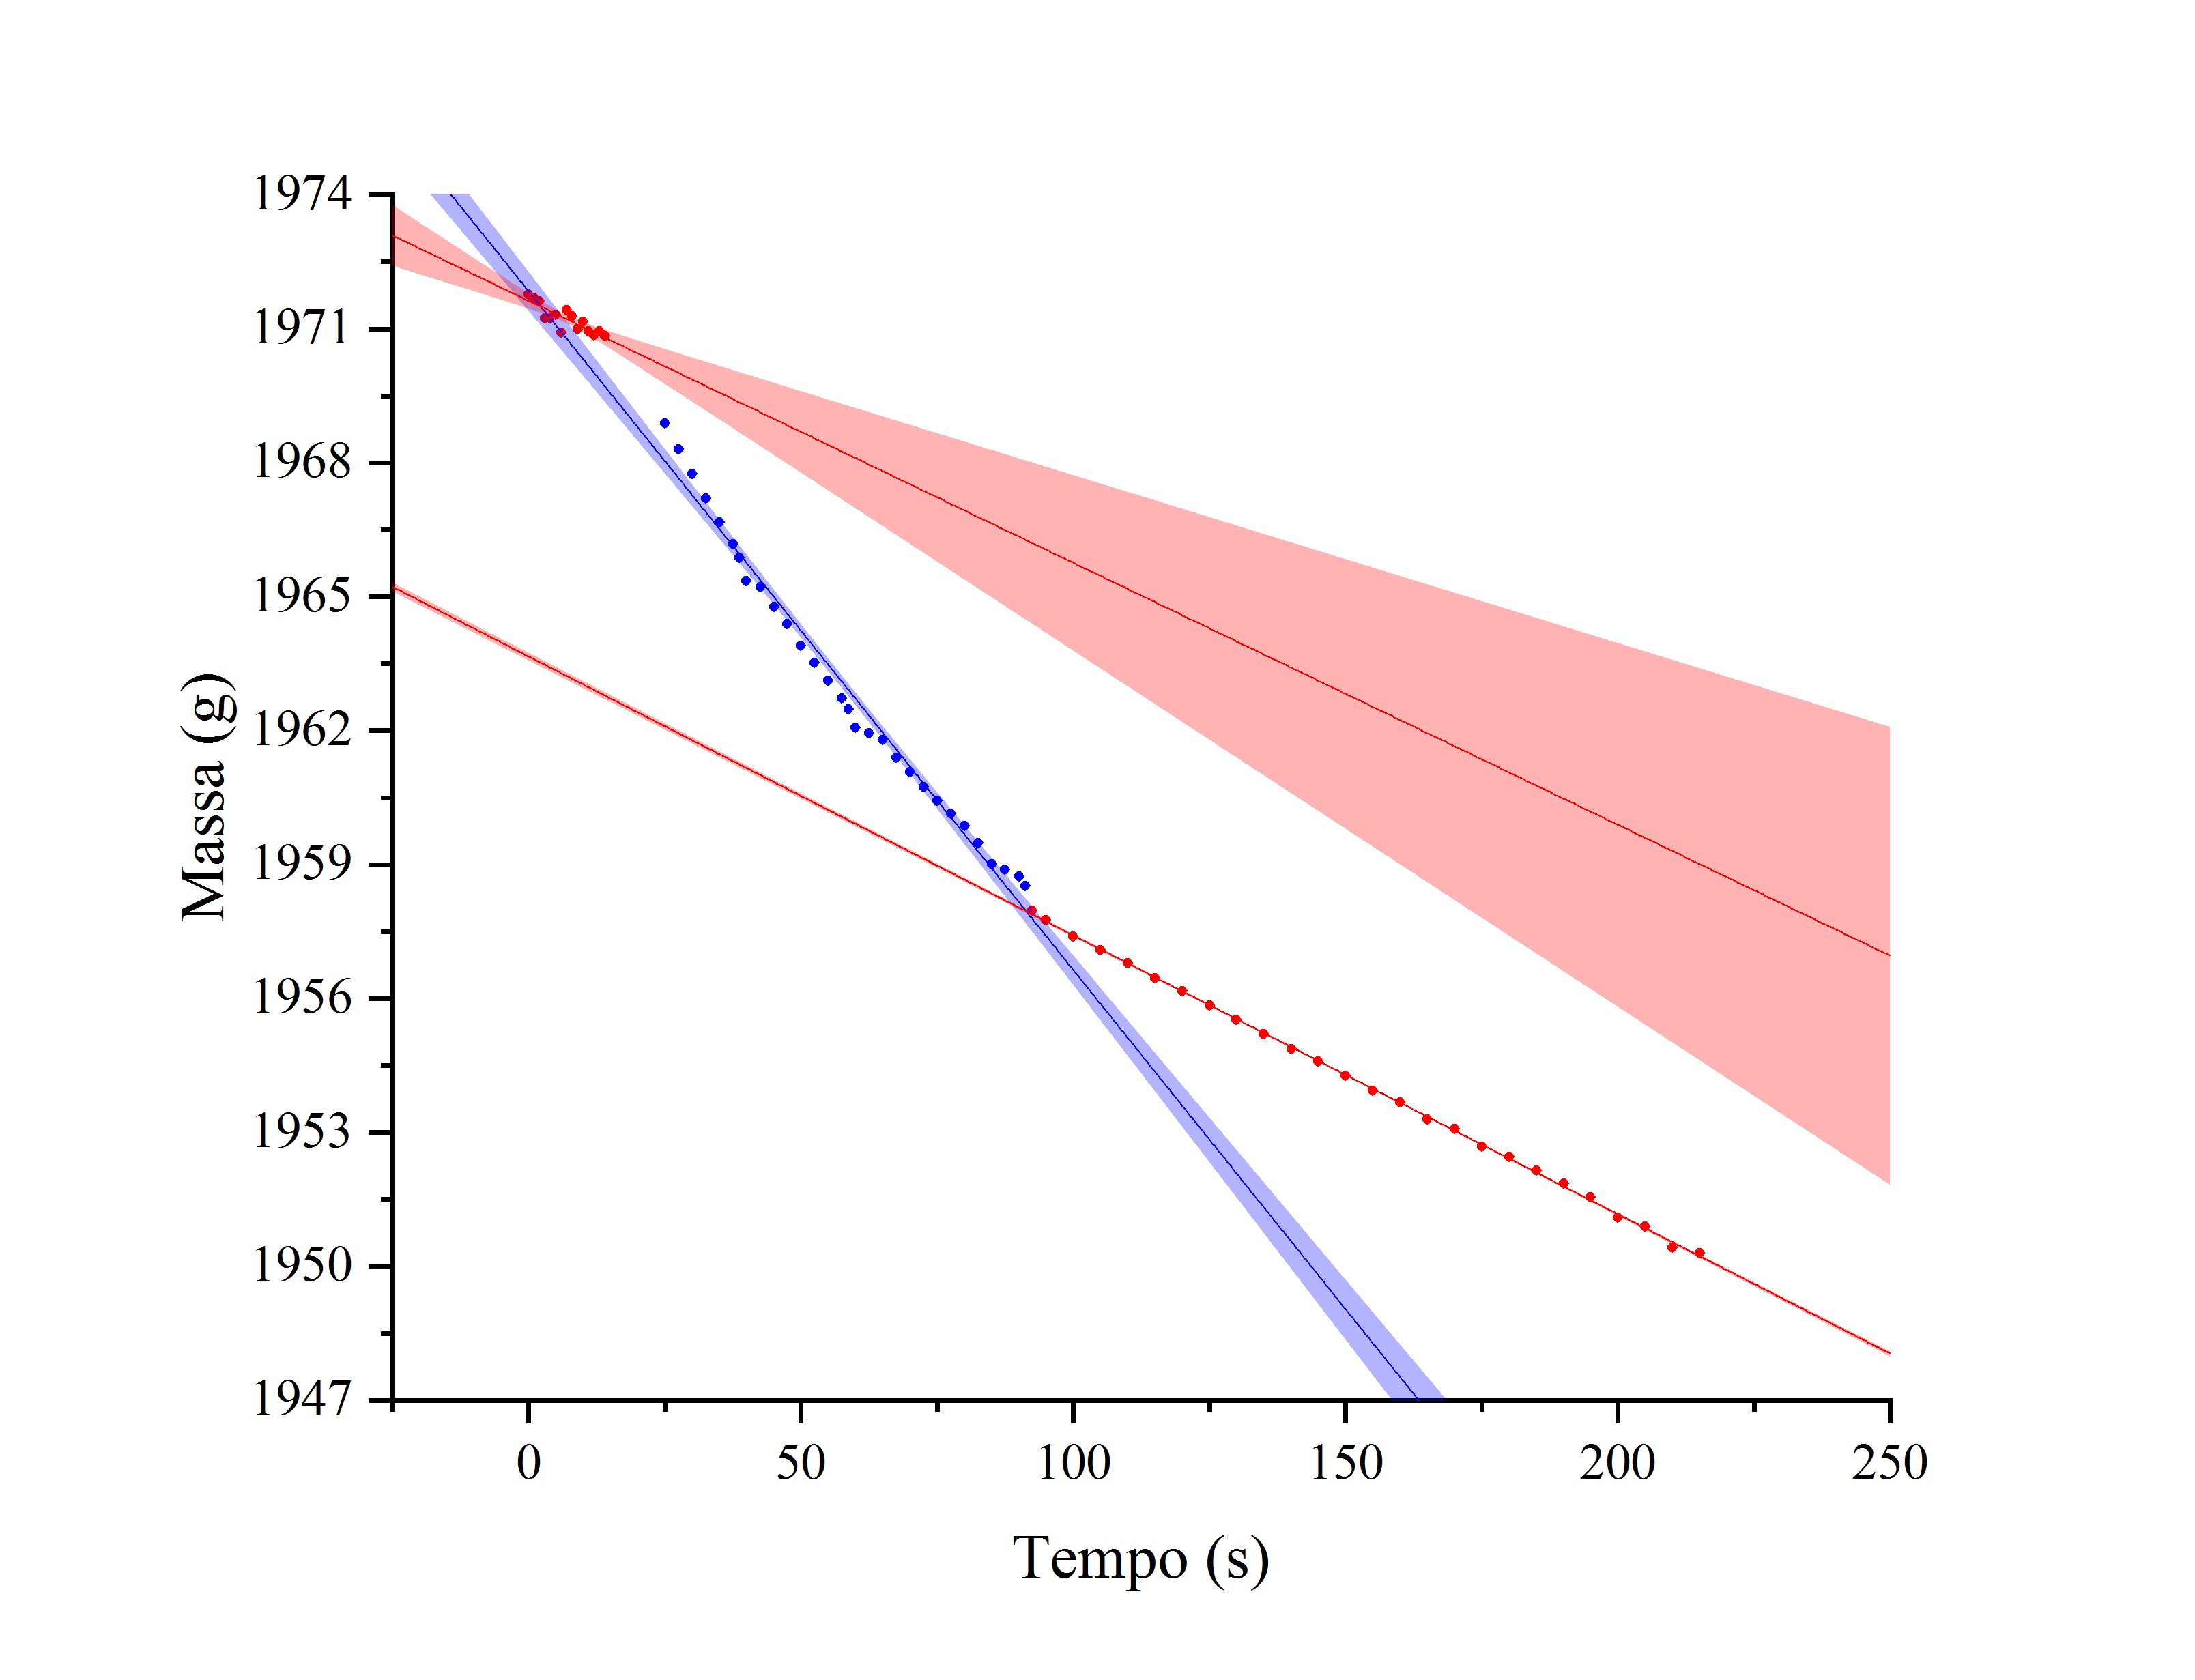
\includegraphics[trim={2cm 0.6cm 3.5cm 1cm},clip,width=.49\textwidth]{img/g_alluminio.png}}\hfil
  \subfloat[][
    Campione $\nabla$ (rame) \\
    $\gamma=(-63.1\pm0.5)\cdot10^{-6}\,\unit{kg\per s}$ \\
    $\Delta t = (74\pm4)\,\unit{s}$
  ]{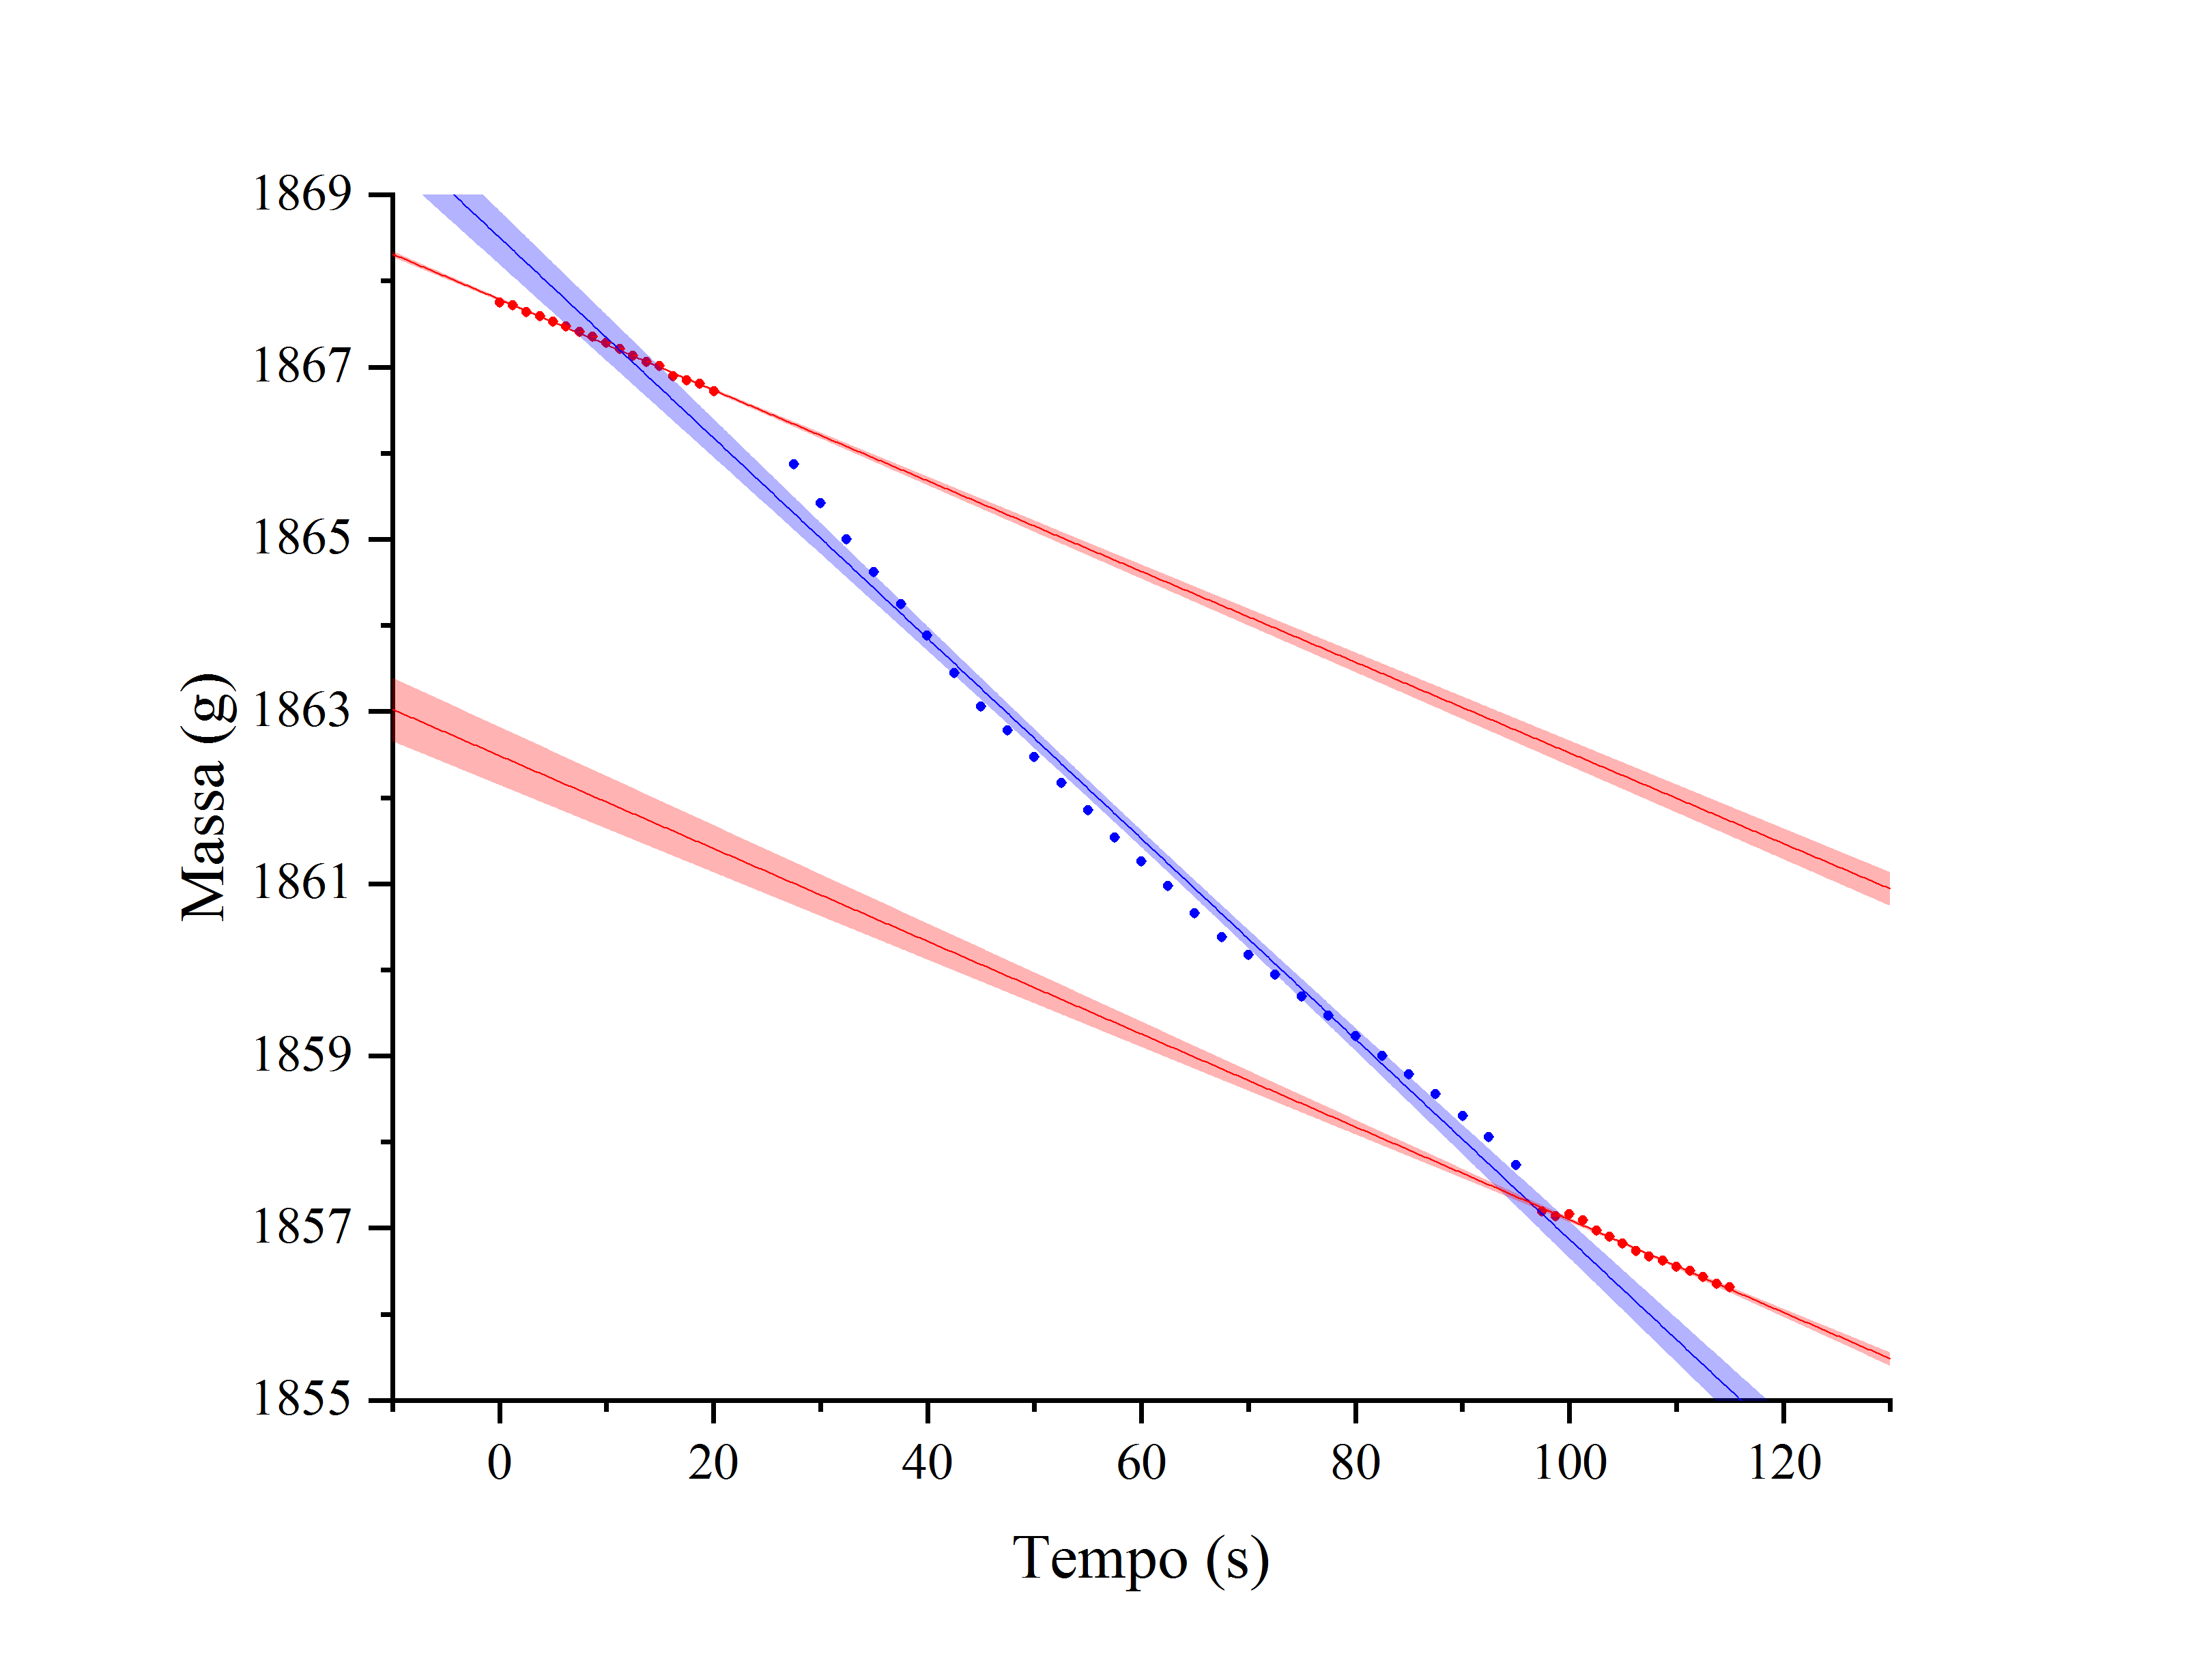
\includegraphics[trim={2cm 0.6cm 3.5cm 1cm},clip,width=.49\textwidth]{img/g_rame.png}}\hfil
\end{figure}

Riportiamo ora, per ogni campione, il valore di $c$ calcolato ($c_\text{mis}$),
accompagnato dalla relativa massa ($\mu$), a confronto con quello atteso
($c_\text{att}$).

\vspace{2mm}
\emph{
  \textbf{Nota.} Per il calcolo di $c$ abbiamo sempre utilizzato
  $\lambda_\text{\emph{vap}}=\lambda_\text{\emph{vap,chiuso}}$: infatti,
  non essendo quest'ultimo compatibile con
  $\lambda_\text{\emph{vap,atteso}}$, esso tiene conto degli errori
  sistematici legati all'aver lasciato chiuso il foro nel
  coperchio del calorimetro.
}

\begin{center}
\begin{tblr}{ |c|c|c|c|c| }
  \hline
    & Materiale & $\mu\;(\unit{g})$
    & $c_\text{mis}\;(\unit{J\,kg^{-1}\,K^{-1}})$
    & $c_\text{att}\;(\unit{J\,kg^{-1}\,K^{-1}})$ \\
  \hline
  $\Xi$ & Piombo & $15.55\pm0.01$ & $107\pm30$ & $130\pm1$ \\
  \hline[dashed]
  $\Delta$ & Ottone & $28.73\pm0.01$ & $391\pm53$ & $377\pm1$ \\
  \hline[dashed]
  $\aleph$ & Alluminio & $10.46\pm0.01$ & $876\pm62$ & $880\pm1$ \\
  \hline[dashed]
  $\nabla$ & Rame & $27.25\pm0.01$ & $408\pm44$ & $385\pm1$ \\
  \hline
\end{tblr}
\end{center}

\subsection{Conclusioni}

Come è possibile osservare facilmente dai dati sopra
riportati, per tutti i campioni $c_\text{mis}$ è risultato
abbondantemente compatibile con $c_\text{att}$.

Possiamo pertanto concludere che l'esperienza ha avuto successo.

\end{document}
